\UseRawInputEncoding
\documentclass{article}
\usepackage[utf8]{inputenc}
\usepackage[french]{babel}
\usepackage{listings}
\usepackage{xcolor}
\usepackage{graphicx}
\usepackage{amsmath}
\usepackage{hyperref}
\usepackage{float}
\usepackage{xurl}
\usepackage{microtype}
\usepackage{enumitem}
\usepackage{parskip}
\usepackage{subcaption}

\definecolor{codegreen}{rgb}{0,0.6,0}
\definecolor{codegray}{rgb}{0.5,0.5,0.5}
\definecolor{codepurple}{rgb}{0.58,0,0.82}
\definecolor{backcolour}{rgb}{0.95,0.95,0.92}

\lstdefinestyle{mystyle}{
    backgroundcolor=\color{backcolour},
    commentstyle=\color{codegreen},
    keywordstyle=\color{magenta},
    numberstyle=\tiny\color{codegray},
    stringstyle=\color{codepurple},
    basicstyle=\ttfamily\footnotesize,
    breakatwhitespace=false,
    breaklines=true,
    captionpos=b,
    keepspaces=true,
    numbers=left,
    numbersep=5pt,
    showspaces=false,
    showstringspaces=false,
    showtabs=false,
    tabsize=2
}

\lstset{style=mystyle}

\title{Rapport d'analyse : Génération et visualisation de distributions statistiques}
\author{Groupe 3 \\ \\ PINCAUD Steve, SAVIARD Matthieu et CHARONNET Henri}
\date{\today}

\begin{document}

\maketitle

\begin{abstract}
Ce rapport présente une implémentation en Python pour générer et visualiser les distributions statistiques suivantes : uniforme entière, uniforme réelle, normale, exponentielle et Poisson. L'objectif est d'analyser le comportement de ces distributions en fonction de la taille de l'échantillon, à l'aide d'histogrammes.
\end{abstract}

\tableofcontents

\section{Introduction}
\sloppy
Ce TP vise à modéliser et visualiser des distributions statistiques fondamentales en utilisant les bibliothèques \texttt{numpy} et \texttt{matplotlib}. L'implémentation repose sur une architecture orientée objet, avec une classe de base \texttt{Distribution} et des sous-classes pour chaque type de distribution. Les histogrammes générés permettent d'observer la convergence des échantillons vers les distributions théoriques lorsque la taille de l'échantillon augmente.

\section{Prérequis}
Pour exécuter ce code, les éléments suivants sont nécessaires :
\begin{itemize}[leftmargin=*]
    \item \textbf{Python 3.12} : Langage de programmation utilisé.
    \item \textbf{Bibliothèques} :
    \begin{itemize}[leftmargin=*]
        \item \texttt{numpy} : Pour la génération de nombres aléatoires et les opérations numériques.
        \item \texttt{matplotlib} : Pour la visualisation des histogrammes.
    \end{itemize}
    \item \textbf{Environnement} : Le code peut être exécuté dans n'importe quel environnement Python.
    La \textbf{seed} utilisée dans l'ensemble des exercices est $\text{seed} = 3$,
    correspondant au numéro du groupe. Cela garantit la reproductibilité des résultats :
    une même seed produit toujours la même séquence pseudo-aléatoire.
\end{itemize}

\section{Première phase du TP}
Pour \textbf{illustrer} notre travail lors de la première partie de ce TP, nous avons choisi de vous présenter une seule de nos implémentations.

\subsection{Exercice 1}
\subsubsection{Objectif}
Ce programme implémente un générateur congruentiel linéaire (GCL), un algorithme simple utilisé pour générer des suites de nombres pseudo-aléatoires. Il compare deux formules différentes et visualise les résultats.

\subsubsection{Architecture du code}
\begin{lstlisting}[language=Python, caption=Implémentation de la fonction générateur congruentiel linéaire (gcl)]
def gcl(x0, a, c, m, n=50):
    x = x0
    resultats = []
    for _ in range(n):
        x = (a * x + c) % m
        resultats.append(x / m)
    return resultats
\end{lstlisting}
\begin{itemize}[leftmargin=*, noitemsep]
    \item \textbf{Paramètres} :
    \begin{itemize}[leftmargin=*, noitemsep]
        \item \texttt{x0} : Valeur initiale (graine).
        \item \texttt{a, c, m} : Coefficients de la formule de récurrence.
        \item \texttt{n} : Nombre d’itérations (par défaut, 50).
    \end{itemize}
    \item \textbf{Fonctionnement} :
    \begin{itemize}[leftmargin=*, noitemsep]
        \item À chaque itération, calcule : \( x = (a \times x + c) \mod m \).
        \item Normalise les résultats en divisant par \( m \) pour obtenir des valeurs dans l’intervalle \([0, 1)\).
        \item Retourne une liste de \( n \) valeurs normalisées.
    \end{itemize}
\end{itemize}

\subsubsection{Formules testées}
\begin{itemize}[leftmargin=*, noitemsep]
    \item \textbf{Formule 1} : \( x_n = 3 \times x_{n-1} \mod 150 \) \\
    Appel : \texttt{gcl(x0=5, a=3, c=0, m=150)}
    \item \textbf{Formule 2} : \( x_n = (5 \times x_{n-1} + 7) \mod 200 \) \\
    Appel : \texttt{gcl(x0=3, a=5, c=7, m=200)}
\end{itemize}

\subsubsection{Visualisation}
Utilise \texttt{matplotlib} pour afficher deux graphiques côte à côte :
\begin{itemize}[leftmargin=*, noitemsep]
    \item \textbf{Gauche} : Évolution des valeurs pour la Formule 1.
    \item \textbf{Droite} : Évolution des valeurs pour la Formule 2.
\end{itemize}
Chaque graphique montre les valeurs en fonction des itérations, avec des points reliés par des lignes (\texttt{'o-'}).

\subsubsection{Analyse et résultat}
Les graphiques permettent de visualiser la périodicité des suites générées. Selon les paramètres \texttt{a, c, m}, les suites peuvent être plus ou moins aléatoires ou cycliques.

\begin{figure}[H]
    \centering
    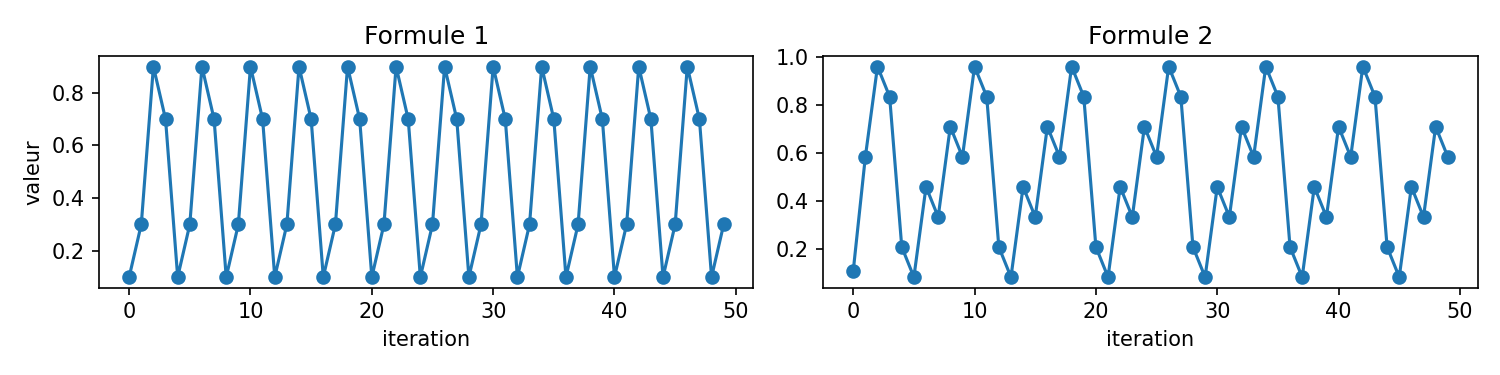
\includegraphics[width=1\linewidth]{Exercice1_Figure.png}
    \caption{Graphiques obtenus lors de l'exécution du code de l'exercice 1}
    \label{fig:exercice1}
\end{figure}

\subsection{Exercice 2}
\subsubsection{Objectif}
Cet exercice vise à simuler une variable aléatoire discrète \( X \) suivant une loi de Bernoulli de paramètre \( p = \frac{1}{3} \). L'objectif est de vérifier la convergence empirique de la proportion de succès (\( X = 1 \)) vers la probabilité théorique \( \frac{1}{3} \) lorsque la taille de l'échantillon \( n \) augmente.

\subsubsection{Architecture du code}
\begin{lstlisting}[language=Python, caption=Simulation d'une loi de Bernoulli avec \( p = \frac{1}{3} \)]
import numpy as np

rng = np.random.default_rng(seed=3)
for n in [100, 1000, 10000]:
    U = rng.uniform(0, 1, size=n)
    X = np.where(U < 1/3, 1, 2)
    prop = np.mean(X == 1)
    print(f"n={n:6d} : proportion X=1 = {prop:.4f}  (théorique : 0.3333)  erreur = {abs(prop - 1/3):.4f}")
\end{lstlisting}

\subsubsection{Description du code}
\begin{itemize}[leftmargin=*, noitemsep]
    \item \textbf{Initialisation} :
    \begin{itemize}[leftmargin=*, noitemsep]
        \item \texttt{rng = np.random.default_rng(seed=3)} : Initialise un générateur de nombres aléatoires avec une graine fixe pour la reproductibilité.
    \end{itemize}
    \item \textbf{Boucle sur les tailles d'échantillon} :
    \begin{itemize}[leftmargin=*, noitemsep]
        \item Pour chaque \( n \) dans \([100, 1000, 10000]\) :
        \begin{itemize}[leftmargin=*, noitemsep]
            \item Génère \( n \) nombres uniformes dans \([0, 1)\) avec \texttt{rng.uniform(0, 1, size=n)}.
            \item Applique la règle : \( X = 1 \) si \( U < \frac{1}{3} \), sinon \( X = 2 \).
            \item Calcule la proportion empirique de \( X = 1 \) avec \texttt{np.mean(X == 1)}.
            \item Affiche la proportion empirique, la valeur théorique (\( \frac{1}{3} \)), et l'erreur absolue entre les deux.
        \end{itemize}
    \end{itemize}
\end{itemize}

\subsubsection{Analyse des résultats}
\begin{itemize}[leftmargin=*, noitemsep]
    \item La proportion empirique de \( X = 1 \) converge vers \( \frac{1}{3} \) lorsque \( n \) augmente.
    \item L'erreur absolue entre la proportion empirique et la valeur théorique diminue avec l'augmentation de \( n \), illustrant la \textbf{loi des grands nombres}.
    \item Exemple de sortie attendue :
    \begin{verbatim}
n=   100 : proportion X=1 = 0.3500  (théorique : 0.3333)  erreur = 0.0167
n=  1000 : proportion X=1 = 0.3340  (théorique : 0.3333)  erreur = 0.0007
n= 10000 : proportion X=1 = 0.3339  (théorique : 0.3333)  erreur = 0.0006
    \end{verbatim}
\end{itemize}

\section{Seconde phase du TP}
\subsection{Architecture du code}
\paragraph{Classe mère : \texttt{Distribution}}
\begin{lstlisting}[language=Python, caption=Implémentation de la classe Distribution mère]
class Distribution:
    """Classe de base représentant une distribution statistique."""

    def __init__(self, name: str, rng: np.random.Generator):
        self.name = name
        self.rng = rng

    def generate(self, n: int) -> np.ndarray:
        raise NotImplementedError("La méthode generate() doit être implémentée dans la sous-classe.")

    def __repr__(self):
        return f"{self.__class__.__name__}(name={self.name!r})"
\end{lstlisting}

La classe \texttt{Distribution} est une classe abstraite qui définit l'interface commune à toutes les distributions. Elle contient :
\begin{itemize}
    \item Un attribut \texttt{name} pour identifier la distribution.
    \item Un générateur aléatoire \texttt{rng} de type \texttt{numpy.random.Generator}.
    \item Une méthode abstraite \texttt{generate(n)} qui doit être implémentée par chaque sous-classe pour générer un échantillon de taille \texttt{n}.
\end{itemize}

\paragraph{Sous-classes de distributions}
Chaque sous-classe hérite de \texttt{Distribution} et implémente la méthode \texttt{generate(n)} selon la distribution spécifique :

\begin{itemize}
    \item \textbf{\texttt{UniformeEntiere}} : Distribution uniforme discrète sur l'intervalle \texttt{[low, high]}. Utilise \texttt{rng.integers}.
    \begin{lstlisting}[language=Python, caption=Implémentation de la classe UniformeEntiere]
class UniformeEntiere(Distribution):
    """Distribution uniforme discrète sur [low, high]."""

    def __init__(self, rng, low: int = 20, high: int = 40):
        super().__init__(f"Uniforme entière ({low}–{high})", rng)
        self.low = low
        self.high = high

    def generate(self, n: int) -> np.ndarray:
        return self.rng.integers(self.low, self.high + 1, size=n)
    \end{lstlisting}

    \item \textbf{\texttt{UniformeReelle}} : Distribution uniforme continue sur l'intervalle \texttt{[low, high)}. Utilise \texttt{rng.uniform}.
    \begin{lstlisting}[language=Python, caption=Implémentation de la classe UniformeReelle]
class UniformeReelle(Distribution):
    """Distribution uniforme continue sur [low, high)."""

    def __init__(self, rng, low: float = 2.0, high: float = 3.0):
        super().__init__(f"Uniforme réelle ({low}–{high})", rng)
        self.low = low
        self.high = high

    def generate(self, n: int) -> np.ndarray:
        return self.rng.uniform(self.low, self.high, size=n)
    \end{lstlisting}

    \item \textbf{\texttt{Normale}} : Distribution normale (gaussienne) avec moyenne \texttt{mu} et écart-type \texttt{sigma}. Utilise \texttt{rng.normal}.
    \begin{lstlisting}[language=Python, caption=Implémentation de la classe Normale]
class Normale(Distribution):
    """Distribution normale (gaussienne)."""

    def __init__(self, rng, mu: float = 0, sigma: float = 0.5):
        super().__init__(f"Normale (µ={mu}, σ={sigma})", rng)
        self.mu = mu
        self.sigma = sigma

    def generate(self, n: int) -> np.ndarray:
        return self.rng.normal(self.mu, self.sigma, size=n)
    \end{lstlisting}

    \item \textbf{\texttt{Exponentielle}} : Distribution exponentielle avec paramètre d'échelle \texttt{scale}. Utilise \texttt{rng.exponential}.
    \begin{lstlisting}[language=Python, caption=Implémentation de la classe Exponentielle]
class Exponentielle(Distribution):
    """Distribution exponentielle."""

    def __init__(self, rng, scale: float = 4):
        super().__init__(f"Exponentielle (moy={scale})", rng)
        self.scale = scale

    def generate(self, n: int) -> np.ndarray:
        return self.rng.exponential(self.scale, size=n)
    \end{lstlisting}

    \item \textbf{\texttt{Poisson}} : Distribution de Poisson avec paramètre \texttt{lam} (λ). Utilise \texttt{rng.poisson}.
    \begin{lstlisting}[language=Python, caption=Implémentation de la classe Poisson]
class Poisson(Distribution):
    """Distribution de Poisson."""

    def __init__(self, rng, lam: float = 42):
        super().__init__(f"Poisson (λ={lam})", rng)
        self.lam = lam

    def generate(self, n: int) -> np.ndarray:
        return self.rng.poisson(self.lam, size=n)
    \end{lstlisting}
\end{itemize}

\paragraph{Classe \texttt{HistogrammeVisualiser}}
Cette classe permet de générer et sauvegarder les histogrammes pour une liste de distributions et une liste de tailles d'échantillons \texttt{ns}. Elle propose une méthode \texttt{tracer()} qui :
\begin{itemize}
    \item Crée une figure avec un sous-graphe par taille d'échantillon.
    \item Génère un histogramme pour chaque distribution et chaque taille d'échantillon.
    \item Sauvegarde les figures au format PNG (optionnel).
    \item Affiche les figures à l'écran (optionnel).
\end{itemize}

\begin{lstlisting}[language=Python, caption=Implémentation de la classe HistogrammeVisualiser]
class HistogrammeVisualiser:
    """Génère et sauvegarde les histogrammes pour une liste de distributions."""

    def __init__(self, distributions: list[Distribution], ns: list[int]):
        self.distributions = distributions
        self.ns = ns

    def tracer(self, save: bool = True, show: bool = True):
        for dist in self.distributions:
            fig, axes = plt.subplots(1, len(self.ns), figsize=(16, 3))
            fig.suptitle(dist.name, fontsize=13)

            for ax, n in zip(axes, self.ns):
                data = dist.generate(n)
                ax.hist(data, bins='auto', edgecolor='white', linewidth=0.4)
                ax.set_title(f"n = {n}")
                ax.set_xlabel("Valeur")
                ax.set_ylabel("Fréquence")

            plt.tight_layout()

            if save:
                filename = f"hist_{dist.name[:10].strip().encode('utf-8').hex()}.png"
                plt.savefig(filename, dpi=150)

            if show:
                plt.show()

            plt.close(fig)
\end{lstlisting}

\subsection{Analyse des résultats}
\subsubsection{Comportement des distributions}
Pour chaque distribution, nous avons généré des histogrammes pour des tailles d'échantillon \( n = 10, 100, 1000, 10000 \). Voici les observations pour chaque type de distribution :

\begin{figure}[H]
    \centering
    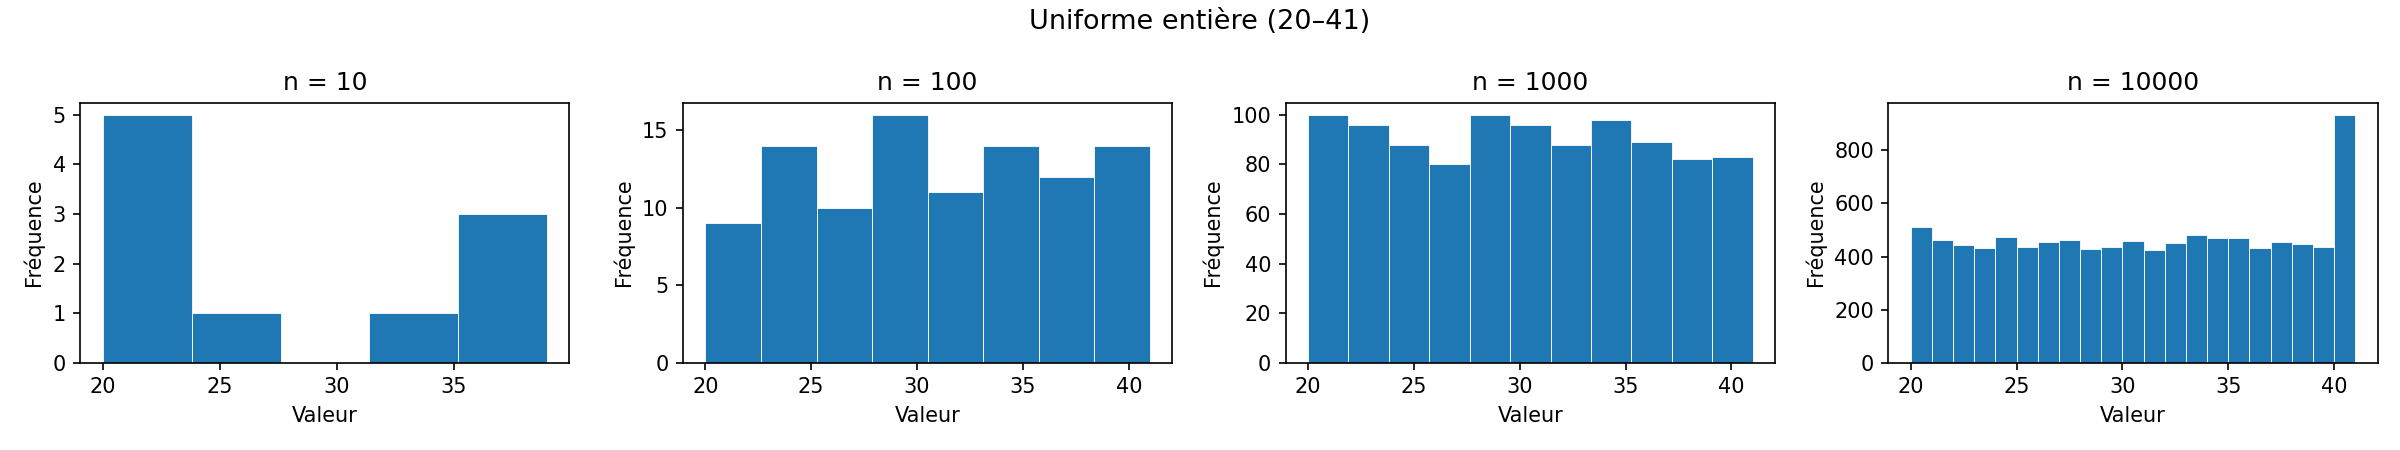
\includegraphics[width=1\linewidth]{hist_556e69666f726d652065.png}
    \caption{Distribution uniforme entière (20–40)}
    \label{fig:uniforme_entiere}
\end{figure}

\begin{figure}[H]
    \centering
    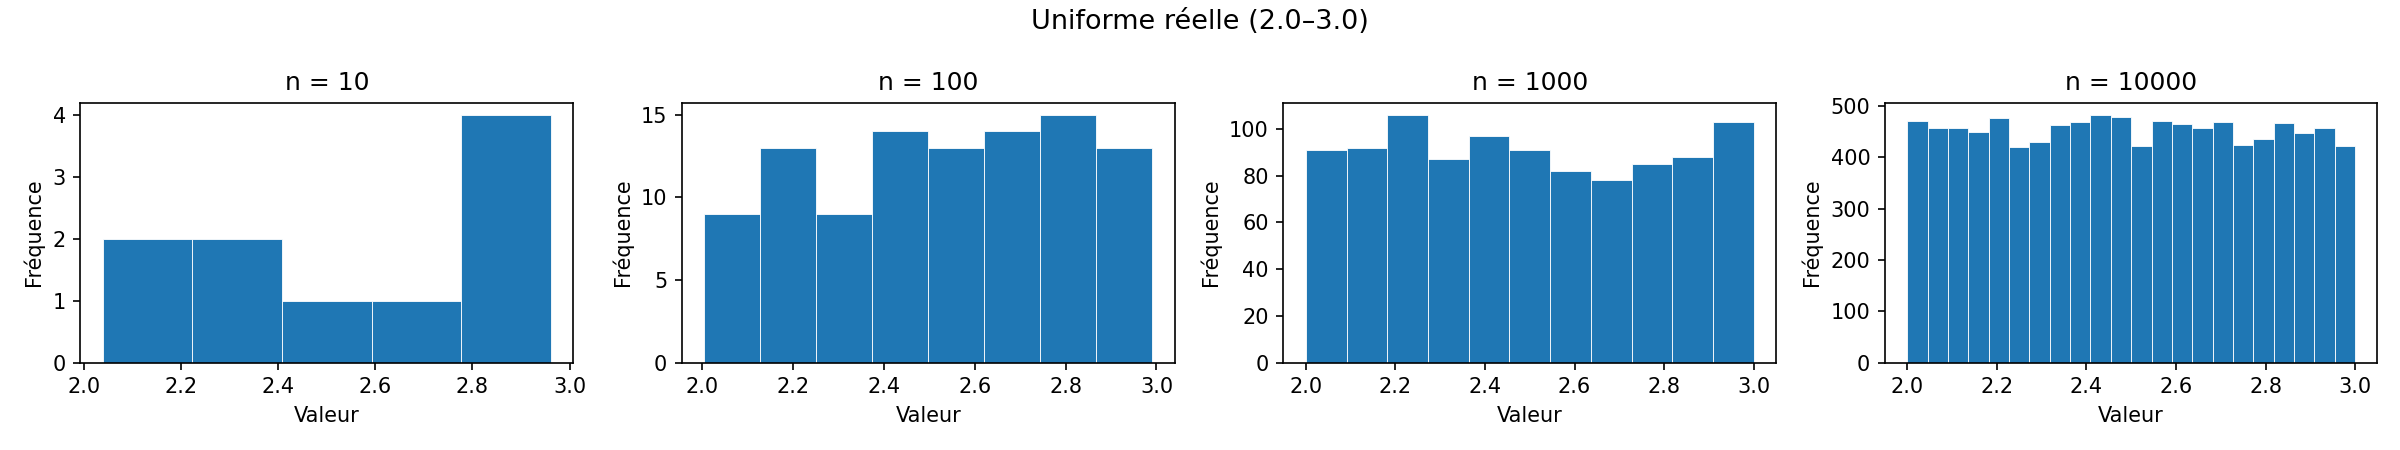
\includegraphics[width=1\linewidth]{hist_556e69666f726d652072.png}
    \caption{Distribution uniforme réelle (2.0–3.0)}
    \label{fig:uniforme_reelle}
\end{figure}

\begin{figure}[H]
    \centering
    \includegraphics[width=1\linewidth]{hist_NORMAL.png}
    \caption{Distribution normale (µ=0, σ=0.5)}
    \label{fig:normale}
\end{figure}

\begin{figure}[H]
    \centering
    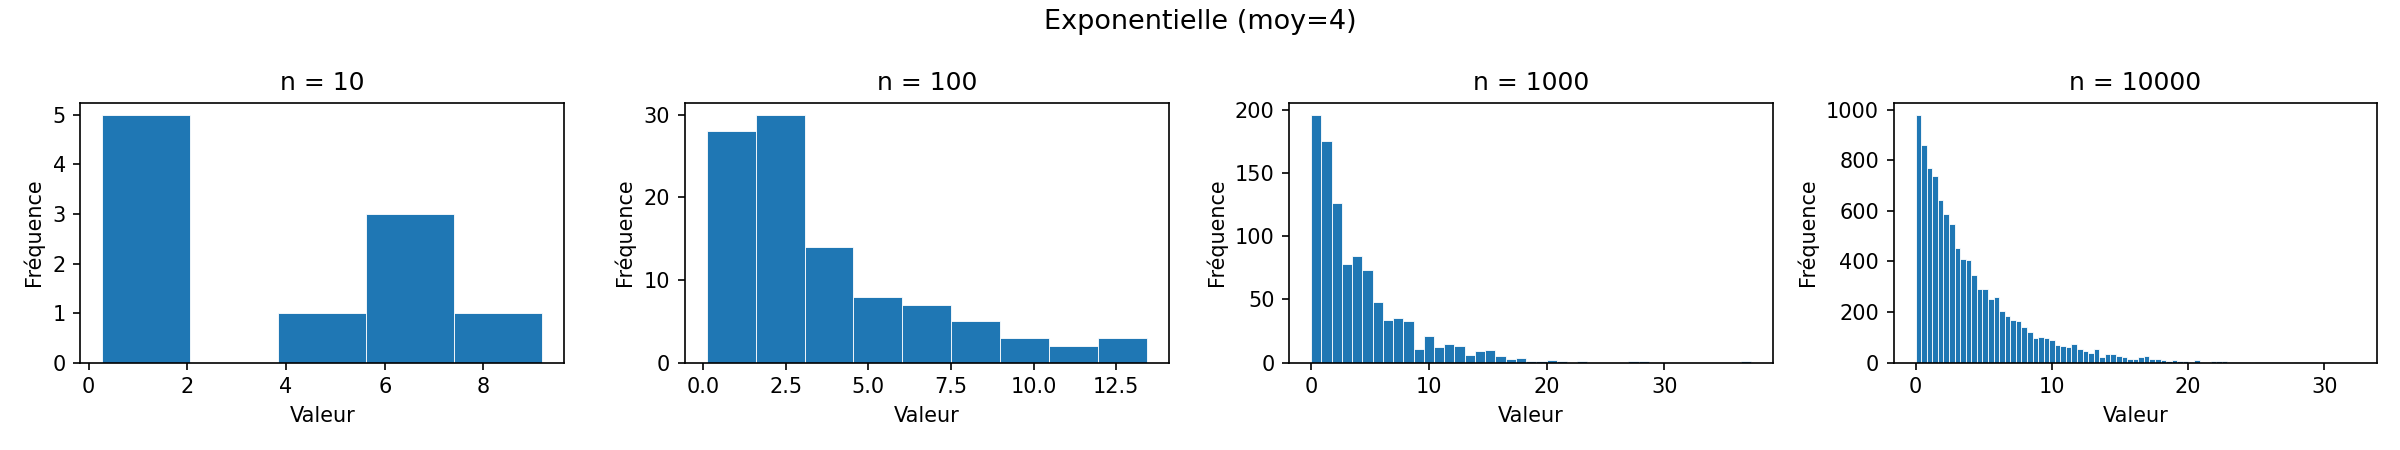
\includegraphics[width=1\linewidth]{hist_4578706f6e656e746965.png}
    \caption{Distribution exponentielle (moy=4)}
    \label{fig:exponentielle}
\end{figure}

\begin{figure}[H]
    \centering
    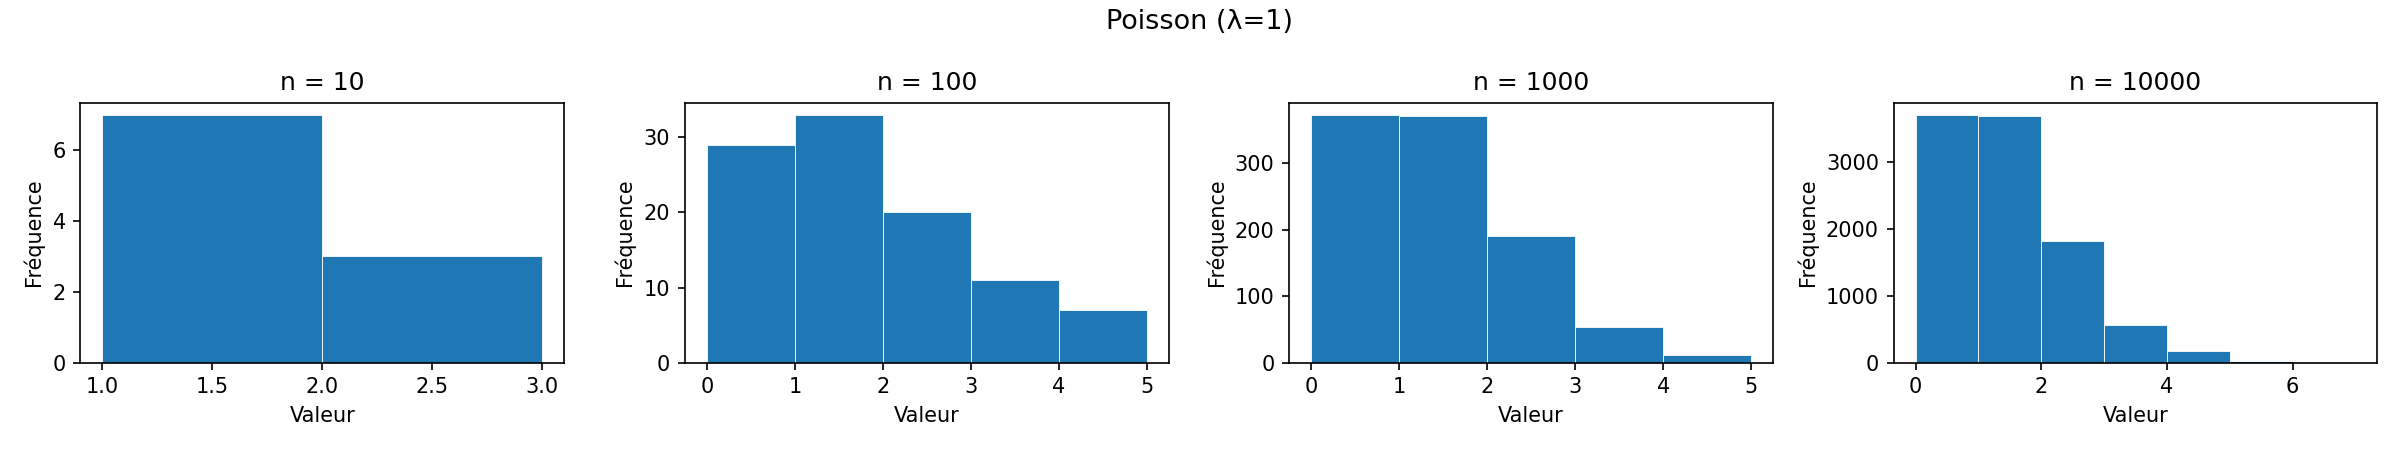
\includegraphics[width=1\linewidth]{hist_Poisson.png}
    \caption{Distribution de Poisson (λ=42)}
    \label{fig:poisson}
\end{figure}

\begin{itemize}[leftmargin=*, noitemsep]
    \item \textbf{Uniforme entière (20–40)} :
    \begin{itemize}[leftmargin=*, noitemsep]
        \item Pour \( n = 10 \), l'histogramme est très irrégulier en raison du faible nombre d'échantillons.
        \item À partir de \( n = 1000 \), la distribution devient uniforme, avec une fréquence presque constante pour chaque valeur entière entre 20 et 40.
        \item Pour \( n = 10000 \), l'histogramme est parfaitement plat, confirmant la propriété d'équiprobabilité de la distribution uniforme discrète.
    \end{itemize}

    \item \textbf{Uniforme réelle (2.0–3.0)} :
    \begin{itemize}[leftmargin=*, noitemsep]
        \item Pour \( n = 10 \), l'histogramme est très bruité.
        \item Dès \( n = 1000 \), la distribution devient visuellement uniforme sur l'intervalle \([2.0, 3.0)\).
        \item Pour \( n = 10000 \), la densité est parfaitement constante, validant la propriété théorique de la distribution uniforme continue.
    \end{itemize}

    \item \textbf{Normale (µ=0, σ=0.5)} :
    \begin{itemize}[leftmargin=*, noitemsep]
        \item Même pour \( n = 100 \), la forme en cloche caractéristique de la distribution normale commence à apparaître.
        \item Pour \( n = 1000 \) et \( n = 10000 \), l'histogramme se rapproche de plus en plus de la courbe théorique de la loi normale, centrée en 0 avec un écart-type de 0.5.
        \item La convergence est rapide, grâce à la nature symétrique et concentrée de cette distribution.
    \end{itemize}

    \item \textbf{Exponentielle (moy=4)} :
    \begin{itemize}[leftmargin=*, noitemsep]
        \item Pour \( n = 10 \), l'histogramme est très irrégulier, avec des valeurs étalées.
        \item À partir de \( n = 1000 \), la décroissance exponentielle caractéristique devient visible, avec une concentration de valeurs proches de 0.
        \item Pour \( n = 10000 \), l'histogramme épouse parfaitement la forme théorique \( f(x) = \frac{1}{4} e^{-x/4} \), confirmant la propriété de mémoire sans vieillissement de la loi exponentielle.
    \end{itemize}

    \item \textbf{Poisson (λ=42)} :
    \begin{itemize}[leftmargin=*, noitemsep]
        \item Pour \( n = 10 \), l'histogramme est très dispersé et peu informatif.
        \item Dès \( n = 1000 \), une forme en cloche asymétrique apparaît, centrée autour de \( \lambda = 42 \).
        \item Pour \( n = 10000 \), l'histogramme se rapproche de la distribution théorique de Poisson, avec un pic à 42 et une queue vers les valeurs supérieures.
        \item La variance empirique se rapproche de la moyenne (42), comme attendu pour une loi de Poisson.
    \end{itemize}
\end{itemize}

\subsubsection{Convergence et loi des grands nombres}
\begin{itemize}[leftmargin=*, noitemsep]
    \item Pour toutes les distributions, on observe une convergence des histogrammes vers leur forme théorique lorsque \( n \) augmente.
    \item Ce comportement illustre la loi des grands nombres, qui stipule que la moyenne empirique d'un échantillon converge vers l'espérance théorique lorsque la taille de l'échantillon tend vers l'infini.
    \item Les histogrammes pour \( n = 10000 \) sont très proches des densités de probabilité théoriques, validant ainsi l'implémentation des générateurs aléatoires.
    \item Les écarts observés pour \( n = 10 \) ou \( n = 100 \) sont normaux et reflètent la variabilité d'échantillonnage, qui diminue avec l'augmentation de \( n \).
\end{itemize}

\section{Annexes}
\subsubsection{Exercice 1}
\begin{lstlisting}[language=Python, caption=Code complet de l'exercice 1]
import matplotlib.pyplot as plt

def gcl(x0, a, c, m, n=50):
    x = x0
    resultats = []
    for _ in range(n):
        x = (a * x + c) % m
        resultats.append(x / m)
    return resultats

f1 = gcl(x0=5, a=3, c=0, m=150)
f2 = gcl(x0=3, a=5, c=7, m=200)

plt.figure(figsize=(12, 4))

plt.subplot(1, 2, 1)
plt.plot(f1, 'o-')
plt.title("Formule 1")
plt.xlabel("iteration")
plt.ylabel("valeur")

plt.subplot(1, 2, 2)
plt.plot(f2, 'o-')
plt.title("Formule 2")
plt.xlabel("iteration")

plt.tight_layout()
plt.show()
\end{lstlisting}

\subsubsection{Exercice 2}
\begin{lstlisting}[language=Python, caption=Code complet de l'exercice 2]
import numpy as np

rng = np.random.default_rng(seed=3)

for n in [100, 1000, 10000]:
    U = rng.uniform(0, 1, size=n)
    X = np.where(U < 1/3, 1, 2)
    prop = np.mean(X == 1)
    print(f"n={n:6d} : proportion X=1 = {prop:.4f}  (théorique : 0.3333)  erreur = {abs(prop - 1/3):.4f}")
\end{lstlisting}

\subsubsection{Phase de groupe}
\begin{lstlisting}[language=Python, caption=Code complet du TP de groupe]
import numpy as np
import matplotlib.pyplot as plt

class Distribution:
    """Classe de base représentant une distribution statistique."""

    def __init__(self, name: str, rng: np.random.Generator):
        self.name = name
        self.rng = rng

    def generate(self, n: int) -> np.ndarray:
        raise NotImplementedError("La méthode generate() doit être implémentée dans la sous-classe.")

    def __repr__(self):
        return f"{self.__class__.__name__}(name={self.name!r})"

class UniformeEntiere(Distribution):
    """Distribution uniforme discrète sur [MIN, MAX]."""

    def __init__(self, rng, low: int = 20, high: int = 41):
        super().__init__(f"Uniforme entière ({low}–{high})", rng)
        self.low = low
        self.high = high

    def generate(self, n: int) -> np.ndarray:
        return self.rng.integers(self.low, self.high + 1, size=n)

class UniformeReelle(Distribution):
    """Distribution uniforme continue sur [MIN, MAX)."""

    def __init__(self, rng, low: float = 2.0, high: float = 3.0):
        super().__init__(f"Uniforme réelle ({low}–{high})", rng)
        self.low = low
        self.high = high

    def generate(self, n: int) -> np.ndarray:
        return self.rng.uniform(self.low, self.high, size=n)

class Normale(Distribution):
    """Distribution normale (gaussienne)."""

    def __init__(self, rng, mu: float = 0, sigma: float = 0.5):
        super().__init__(f"Normale (µ={mu}, σ={sigma})", rng)
        self.mu = mu
        self.sigma = sigma

    def generate(self, n: int) -> np.ndarray:
        return self.rng.normal(self.mu, self.sigma, size=n)

class Exponentielle(Distribution):
    """Distribution exponentielle."""

    def __init__(self, rng, scale: float = 4):
        super().__init__(f"Exponentielle (moy={scale})", rng)
        self.scale = scale

    def generate(self, n: int) -> np.ndarray:
        return self.rng.exponential(self.scale, size=n)

class Poisson(Distribution):
    """Distribution de Poisson."""

    def __init__(self, rng, lam: float = 42):
        super().__init__(f"Poisson (λ={lam})", rng)
        self.lam = lam

    def generate(self, n: int) -> np.ndarray:
        return self.rng.poisson(self.lam, size=n)

class HistogrammeVisualiser:
    """Génère et sauvegarde les histogrammes pour une liste de distributions."""

    def __init__(self, distributions: list[Distribution], ns: list[int]):
        self.distributions = distributions
        self.ns = ns

    def tracer(self, save: bool = True, show: bool = True):
        for dist in self.distributions:
            fig, axes = plt.subplots(1, len(self.ns), figsize=(16, 3))
            fig.suptitle(dist.name, fontsize=13)

            for ax, n in zip(axes, self.ns):
                data = dist.generate(n)
                ax.hist(data, bins='auto', edgecolor='white', linewidth=0.4)
                ax.set_title(f"n = {n}")
                ax.set_xlabel("Valeur")
                ax.set_ylabel("Fréquence")

            plt.tight_layout()

            if save:
                filename = f"hist_{dist.name[:10].strip().encode('utf-8').hex()}.png"
                plt.savefig(filename, dpi=150)

            if show:
                plt.show()

            plt.close(fig)

if __name__ == "__main__":
    print("+++ START TP1 Main ...")
    rng = np.random.default_rng(seed=3)

    distributions = [
        UniformeEntiere(rng),
        UniformeReelle(rng),
        Normale(rng),
        Exponentielle(rng),
        Poisson(rng),
    ]

    ns = [10, 100, 1000, 10000]

    visualiseur = HistogrammeVisualiser(distributions, ns)
    visualiseur.tracer(save=True, show=True)

    print("+++ END TP1 Main.")
\end{lstlisting}

\end{document}